\newpage
\section{Opis implementacji systemu}

\subsection{Framework}
Framework
Narzędziem użytym w realizacji projektu jest JADE 4.5.0 (Java Agent Development Framework). Jest to popularny framework przeznaczony do implementowania systemów wieloagentowych w pełni zaimplementowany w języku Java. Wybraliśmy JADE, ponieważ jak można przeczytać w dokumentacji:

\begin{itemize}
\item w JADE wdrożony został pełny model komunikacji FIPA, a jego komponenty zostały wyraźnie wyróżnione i w pełni zintegrowane: protokoły interakcji, koperta, ACL, języki treści, schematy kodowania, ontologie i protokoły transportowe. 

\item architektura komunikacji oferuje elastyczne i wydajne przesyłanie wiadomości, gdzie JADE tworzy i zarządza kolejką przychodzących wiadomości ACL. Agenci mogą uzyskać dostęp do swojej kolejki za pomocą kombinacji kilku trybów: blokowania, odpytywania, limitu czasu i dopasowywania wzorców. 

\item Dodatkowo przydatną funkcjonalnością jest możliwość sterowania konfiguracją za pomocą interfejsu GUI. 
\end{itemize}

\subsection{Sposób implementacji agentów}
Utworzyliśmy dwie klasy agentów CarAgent oraz ParkingAgent. Każdy agent dziedziczy funkcjonalność po klasie jade.core.Agent. Agenty wykorzystują klasę jade.core.behaviours.
Behaviour do implementacji aktywności oraz protokołów zdefiniowanych dla ról. 

\textbf{CarAgent} - Agent samochód, który może się przemieszczać. Dla celów testowych przyjęliśmy, iż na początku swojego istnienia agent ten losuje swoją pozycję początkową na mapie i dodaje zachowania UpdateListOfParkings, CallForParkingOffers, SendReservationInfo oraz ReservationCancellation, ListenForLocationCancelSubscriptionFromCarTracker.

\textit{UpdateListOfParkings} - służy do  wysyłania zapytania do wszystkich parkingów z prośbą o informacje o ich lokalizacji i uaktualnienia ich położenia. Protokół ten jest aktywowany na początku istnienia agenta samochodu. Agent zapisuje położenia wszystkich parkingów w HashMapie, gdzie kluczem jest AID parkingu, a wartością jest lokalizacja parkingu. Lokalizacje wszystkich parkingów są niezbędne dla CarAgent, ponieważ chce on wiedzieć, który parking dysponujący wolnym miejscem znajduje się najbliżej. 

\textit{CallForParkingOffers} - służy do zapoczątkowania konwersacji z najbliższymi parkingami w celu zarezerwowania miejsca. Agent samochód wysyła wiadomość typu CFP i otrzymuje od parkingów posiadających wolne miejsce odpowiedź typu PROPOSE lub REFUSE. Następnie typowany jest najbliższy parking z wolnym miejscem i podejmowana jest próba dokonania rezerwacji miejsca (ACCEPT PROPOSAL). Jeżeli CarAgent otrzyma odpowiedź pozytywną (INFORM) od ParkingAgent, to dany parking jest zapisany w pamięci jako cel podróży, jeżeli jednak otrzymamy odpowiedź negatywną (FAILURE) to ponownie rozpoczynamy protokół CallForParkingOffers.

\textit{SendReservationInfo} - służy do wysłania wiadomości od CarAgent (INFORM) do ParkingAgent o rezerwacji zrobionej dla konkretnego agenta. Po otrzymaniu informacji ParkingAgent wysyła potwierdzenie CONFIRM.

\textit{CancelClientReservation} - służy do wysłania wiadomości o rezygnacji z zarezerwowanego miejsca (CANCEL) do ParkingAgent, będącego do tej pory celem podróży agenta-samochodu (CarAgent). Po otrzymaniu takiego żądania ParkingAgent zwalnia miejsce postojowe, a następnie wysyła potwierdzenie wykonania akcji (CONFIRM).

\textit{ListenForLocationCancelSubscriptionFromCarTracker} - służy do nasłuchiwania czy CarTracker chce przestać subskrybować wiadomości, które są wysyłane w protokole SendReservationInfo.


\textbf{ParkingAgent} - agent parking posiadający miejsca parkingowe udostępniane pojazdom. Głównym zadaniem agenta jest oferowanie wolnych miejsc parkingowych oraz śledzenie aktualnej pozycji samochodów posiadających rezerwację. Agent ten wykorzystuje zachowania:

\textit{SendCoordinates} - służy do wysłania informacji o swojej pozycji. Zachowanie to jest cykliczne i wykonywane po otrzymaniu wiadomości od agenta samochodu typu INFORM\_REF.

\textit{SendAvailablePlaceInfo} - zachowanie to jest cykliczne, wykonywane po przyjściu wiadomości zawierającej performatywę CFP od CarAgent. Jeżeli agent posiada wolne miejsce parkingowe to wysyła wiadomość typu PROPOSE w odpowiedzi. W przypadku kiedy agent nie posiada wolnego miejsca następuje wysłanie odpowiedzi zawierającej performatywę REFUSE.

\textit{ConfirmReservation} - zachowanie cykliczne; po otrzymaniu od CarAgent wiadomości zawierającej performatywę ACCEPT\_PROPOSAL, wyrażającej chęć zarezerwowania miejsca na danym parkingu, ParkingAgent zmienia stan miejsca z “wolny” na “zajęty” i odsyła wiadomość o pozytywnym przebiegu procesu (INFORM). Jeśli dane miejsce zostanie przed otrzymaniem wiadomości zawierającej ACCEPT\_PROPOSAL zajęte przez innego CarAgent, zostaje wysłana wiadomość informująca o niepowodzeniu rezerwacji (FAILURE).

\textit{ConfirmCancellation} - zachowanie cykliczne, po otrzymaniu wiadomości od CarAgent wyrażającej żądanie usunięcia rezerwacji miejsca parkingowego (CANCEL) zmienia stan miejsca z “zajęty” na “wolny”, a następnie wysyła odpowiedź o powodzeniu akcji (CONFIRM).

\textit{getReservationInfo} - zachowanie cykliczne; służy do odbierania wiadomości od CarAgent o dokonaniu rezerwacji dla tego CarAgenta na parkingu, którym jest adresat wiadomości - ParkingAgent. Po otrzymaniu informacji ParkingAgent przesyła potwierdzenie CONFIRM.


\subsection{Sposób implementacji komunikatów}

\subsubsection{Zastosowane performatywy}
\begin{enumerate}
    \item INFORM\_REF
    \item INFORM
    \item FAILURE
    \item CFP
    \item PROPOSE
    \item ACCEPT\_PROPOSAL
    \item CANCEL
    \item CONFIRM
    \item REFUSE
\end{enumerate}

\subsubsection{Protokoły komunikacyjne}

W trakcie dotychczasowej implementacji został użyty tylko jeden typowy protokół komunikacyjny zdefiniowany przez FIPA i jest nim Subscribe Interaction Protocol, który został zastosowany do śledzenia Car Agents przez rolę CarTracker realizowaną przez Parking Agent. Pozostała wymiana komunikatów pomiędzy agentami została zebrana w indywidualnie zdefiniowanych dla naszego systemu protokołach stworzonych poprzez rozszerzenie klasy Behaviours, CyclicBehaviours oraz TickerBehaviours.

\subsubsection{Zastosowane języki treści}
Zastosowanym językiem treści jest FIPA Semantic Language (SL), który jest standardowo zaimplementowany we frameworku JADE.

\subsection{Wykorzystane standardy}

Implementowany system jest zgodny ze standardami FIPA, ze względu na wykorzystanie frameworka JADE.

\begin{itemize}
\item FIPA ACL (Agent Communication Language)
\item FIPA SL (Semantic Language) - język semantyczny dla komunikacji ACL

\end{itemize}


\subsection{Algorytmy}

Algorytmy wykorzystane w systemie zostały pokrótce opisane w sposobie implementacji agentów. Na uwagę zasługuje sposób implementacji środowiska oraz sposób poruszania się po nim agentów. Stan naszego systemu jest zdefiniowany w postaci mapy 2D, gdzie każda z kratek odpowiada współrzędnej w środowisku agentów. Do każdej współrzędnej mogą być przypisane trzy wartości: czy współrzędna jest ulicą czy parkingiem. Samochody są losowo inicjalizowane na współrzędnych odpowiadających ulicom. Parking docelowy jest znajdowany poprzez obliczanie ścieżek do wszystkich parkingów, a następnie wybranie najkrótszej trasy. Samochód porusza się w jego kierunku po drodze obliczonej w algorytmie wybierania ścieżki (opisanym poniżej). Końcowo samochód wjeżdża na współrzędną z parkingiem. Dopuszcza się możliwość, że dwa samochody znajdują się na tej samej współrzędnej. W aktualnej wersji systemu wszystkie pola mapy są ulicami.

\textbf{Algorytm wyznaczania ścieżki} został zaimplementowany przy pomocy algorytmu przeszukiwania wszerz (BFS). Algorytm ten w formie iteracyjnej wykorzystuje kolejkę do określenia, które kolejne punkty powinniśmy przebadać. Rozpoczynając od punktu startowego dodajemy wszystkie sąsiednie, nieodwiedzone wcześniej, punkty do kolejki i powtarzamy ten proces dla wszystkich punktów w kolejce. Jeżeli dotrzemy do punktu docelowego to zwracamy listę, która jest ścieżką od miejsca początkowego do docelowego. Nie jest to najoptymalniejszy algorytm (u nas, O($ i \cdot j $) time | O($ i \cdot j $) space, gdzie i - szerokość mapy, j - wysokość mapy), jednak został wybrany ze względu na łatwość implementacji w realizowanym systemie.

\newpage
\subsection{Wizualizacja}

Postanowiliśmy zwizualizować działanie naszego projektu poprzez wyświetlanie informacji o aktualnym stanie systemu w konsoli oraz pokazywaniu położenia agentów na mapie 2D. Agent aktualizując swoje położenie wysyła informację do serwera, który przechowuje dane o bieżącym położeniu każdego agenta. Następnie serwer przekazuje uaktualnione informacje do aplikacji React, gdzie wyświetlana jest mapa. Backend i Frontend połączone są ze sobą poprzez websocket, więc wszystkie aktualizacje są wykonywane w czasie rzeczywistym. Ze względu na taki stos technologiczny możliwe są opóźnienia pomiędzy prezentowanym stanem systemu na mapie, a w konsoli. Przykładowa mapa jest widoczna na rysunku \ref{fig:przyklad_mapy}, gdzie kratka: biała oznacza drogę, czerwona parking, a niebieska samochód. Przykładowe wizualizacje naszego systemu są dostępne w postaci gifów na repozytorium naszego projektu w README.

\begin{figure}[H]
    \centering 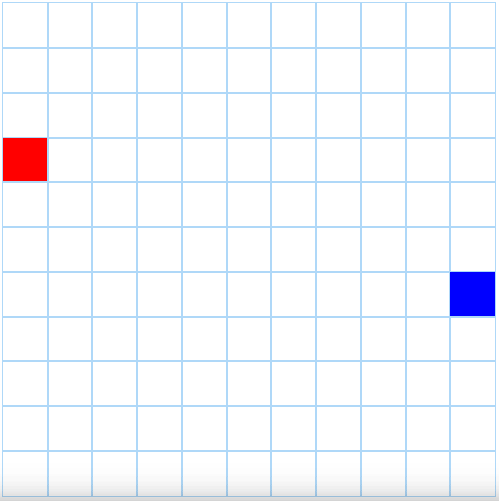
\includegraphics[width=0.7\linewidth]{przyklad_mapy.png}
    \caption{Przykład mapy.}
    \label{fig:przyklad_mapy}
\end{figure}

\newpage
\subsection{Napotkane problemy i zmiany w kolejnej iteracji}
\begin{itemize}
\item Żaden członek zespołu nie jest biegły w Javie, więc dodatkową trudnością  było szybkie zapoznanie się z samym językiem, a nie tylko nowym frameworkiem. Z tego powodu, nie mogliśmy się wyłącznie skupić na najlepszym rozwiązaniu i implementacji problemu.

\item Podczas implementacji równoległego oczekiwania na wiadomości mieliśmy problem z przechwytywaniem wiadomości przez niepowołane do tego zachowania. Problem ten rozwiązaliśmy wykorzystując zaimplementowane w JADE szablony wiadomości (jade.lang.acl.MessageTemplate). Za pomocą metod MatchPerformative, MatchConversationID i wyfiltrowaliśmy przychodzące wiadomości skierowane do poszczególnych zachowań.
\end{itemize}